%% ECON 282E -- Session 4, Deck B1: Function Approximation and Interpolation
%% Ported from QM Lec.4 F59-F68 (bilinear, triangular, cubic spline) and QM Lec.7
%% F20, F24-F26 (Chebyshev nodes, splines, shape preservation, the comparison
%% table).  TWO source errors corrected: linear interpolation DOES preserve
%% concavity, and the Chebyshev nodes come out descending.
%% Numbers from tools/figures/s04_numbers.json, keys "runge",
%% "shape_preservation", "shape_preservation_kinked", "gibbs".

%% ECON 282E -- Foundations of Macroeconomics (UC Riverside, Fall 2026)
%% Shared Beamer preamble for every deck in slides/S01 ... slides/S10.
%%
%% Usage (a deck lives in slides/S0X/ and is compiled from that folder):
%%   %% ECON 282E -- Foundations of Macroeconomics (UC Riverside, Fall 2026)
%% Shared Beamer preamble for every deck in slides/S01 ... slides/S10.
%%
%% Usage (a deck lives in slides/S0X/ and is compiled from that folder):
%%   %% ECON 282E -- Foundations of Macroeconomics (UC Riverside, Fall 2026)
%% Shared Beamer preamble for every deck in slides/S01 ... slides/S10.
%%
%% Usage (a deck lives in slides/S0X/ and is compiled from that folder):
%%   \input{../preamble/course_preamble.tex}
%%   \decktitle{1}{A1}{Who I Am \& Why This Course}{September 24, 2026}
%%   \begin{document}
%%   \makedecktitle
%%   ...
%%
%% Adapted from Courses/AI-ECON-2026/source/shared_preamble.tex (Metropolis theme,
%% concept/caution/example/takeaway boxes, \sectiondivider). Changes for this course:
%%   * course title block (\decktitle / \makedecktitle) instead of \makebeamertitle
%%   * \zh{...} typesets Chinese (book titles) under pdflatex via CJKutf8
%%   * researchbox for the "Research in the wild" frames
%%   * section pages off; TikZ libraries and the course map loaded here
%% Build with pdflatex only (two passes); tools/build_slides.py does this for you.

\documentclass[10pt,english,aspectratio=169]{beamer}

\usepackage[T1]{fontenc}
\usepackage{textcomp}
\usepackage[utf8]{inputenc}
\usepackage{babel}
\usepackage{CJKutf8}

\usepackage{amsmath, amssymb, amsthm, graphicx}
\usepackage{booktabs, multirow, tabularx}
\usepackage{tikz}
\usetikzlibrary{positioning,arrows.meta,shapes,calc,fit,backgrounds}
\usepackage{pgfplots}
\pgfplotsset{compat=1.16}
\usepackage[most]{tcolorbox}
\tcbuselibrary{skins, breakable}
\usepackage{listings}
\usepackage{xcolor}

\lstset{
  basicstyle=\ttfamily\small,
  keywordstyle=\color{blue!80!black}\bfseries,
  commentstyle=\color{green!50!black}\itshape,
  stringstyle=\color{orange!80!black},
  backgroundcolor=\color{gray!8},
  frame=single,
  rulecolor=\color{gray!40},
  breaklines=true,
  showstringspaces=false,
  numbers=none,
}

\usetheme{metropolis}
\usefonttheme{professionalfonts}
\metroset{sectionpage=none}

\definecolor{LightGray}{RGB}{230,230,230}
\definecolor{RedTitle}{RGB}{0,0,200}
\definecolor{VeryLightGray}{RGB}{245,245,245}
\definecolor{DarkText}{RGB}{0,0,0}
\definecolor{UCRBlue}{RGB}{0,45,106}
\definecolor{UCRGold}{RGB}{241,171,0}

% Stage colours of the course arc (used by the course map and elsewhere)
\colorlet{StageTrunk}{blue!12}
\colorlet{StageBranch}{cyan!14}
\colorlet{StageMachine}{gray!18}
\colorlet{StageWall}{red!14}
\colorlet{StageTools}{orange!20}
\colorlet{StageData}{green!16}
\colorlet{StageAgents}{violet!14}

\hypersetup{bookmarks=false,breaklinks=true,pdfborder={0 0 0},colorlinks=true,
  linkcolor=DarkText,urlcolor=RedTitle}

\setbeamercolor{background canvas}{bg=white}
\setbeamercolor{title}{fg=RedTitle}
\setbeamercolor{frametitle}{bg=VeryLightGray,fg=DarkText}
\setbeamercolor{normal text}{fg=DarkText}
\setbeamercolor{alerted text}{fg=RedTitle}
\setbeamersize{text margin left=5mm, text margin right=5mm}
\addtobeamertemplate{frametitle}{}{\vspace{-0.5em}}

\setbeamertemplate{navigation symbols}{}
\setbeamertemplate{footline}{%
  \hspace{5mm}{\usebeamerfont{page number in head/foot}\color{black!45}%
  ECON 282E \,$\cdot$\, \insertshortdeck}\hfill%
  \usebeamercolor[fg]{page number in head/foot}%
  \usebeamerfont{page number in head/foot}%
  \insertframenumber\,/\,\inserttotalframenumber\kern1em\vskip2pt%
}

% ---------------------------------------------------------------------------
% Chinese text under pdflatex (book titles etc.)
\newcommand{\zh}[1]{\begin{CJK*}{UTF8}{gbsn}#1\end{CJK*}}

% ---------------------------------------------------------------------------
% Deck title block
%   \decktitle{session}{deck id}{title}{date}
\newcommand{\insertshortdeck}{}
\newcommand{\decksession}{}
\newcommand{\deckid}{}
\newcommand{\decktitletext}{}
\newcommand{\deckdate}{}
\newcommand{\decktitle}[4]{%
  \renewcommand{\decksession}{#1}%
  \renewcommand{\deckid}{#2}%
  \renewcommand{\decktitletext}{#3}%
  \renewcommand{\deckdate}{#4}%
  \renewcommand{\insertshortdeck}{Session #1 \,$\cdot$\, Deck #1.#2}%
  \title{#3}%
  \author{Zhigang Feng}%
  \date{#4}%
}
\newcommand{\makedecktitle}{%
  \begin{frame}[plain,noframenumbering]
    \begin{tikzpicture}[remember picture,overlay]
      \fill[UCRBlue] (current page.north west) rectangle ([yshift=-0.55cm]current page.north east);
      \fill[UCRGold] ([yshift=-0.55cm]current page.north west) rectangle ([yshift=-0.62cm]current page.north east);
      \node[anchor=west, text=white, font=\small\bfseries] at ([xshift=5mm,yshift=-0.275cm]current page.north west)
        {ECON 282E \,$\cdot$\, Foundations of Macroeconomics};
      \node[anchor=east, text=white, font=\small] at ([xshift=-5mm,yshift=-0.275cm]current page.north east)
        {UC Riverside \,$\cdot$\, Fall 2026};
    \end{tikzpicture}
    \vspace*{1.1cm}
    {\usebeamerfont{title}\color{black!55}\large Session \decksession\ \,$\cdot$\, Deck \decksession.\deckid\par}
    \vspace{0.25cm}
    {\usebeamerfont{title}\color{RedTitle}\LARGE\bfseries \decktitletext\par}
    \vspace{0.7cm}
    {\large Zhigang Feng\par}
    \vspace{0.15cm}
    {\color{black!65}\deckdate\par}
    \vfill
    {\footnotesize\itshape\color{black!55}Build it on paper $\;\to\;$ solve it on the machine $\;\to\;$ push it to the frontier with AI\par}
  \end{frame}}

% ---------------------------------------------------------------------------
% Section divider (plain frame, not counted)
\newcommand{\sectiondivider}[2]{%
\begin{frame}[plain,noframenumbering]
\begin{center}
\vfill
{\Large\textbf{#1}\par}
\vspace{0.35cm}
{\normalsize #2\par}
\vfill
\end{center}
\end{frame}
}

% ---------------------------------------------------------------------------
% Boxes
\newtcolorbox{conceptbox}[1][]{colback=blue!3, colframe=RedTitle!55, boxrule=0.35mm,
  arc=1mm, left=2mm, right=2mm, top=1mm, bottom=1mm, #1}
\newtcolorbox{cautionbox}[1][]{colback=red!3, colframe=red!50!black, boxrule=0.35mm,
  arc=1mm, left=2mm, right=2mm, top=1mm, bottom=1mm, #1}
\newtcolorbox{examplebox}[1][]{colback=green!3, colframe=green!45!black, boxrule=0.35mm,
  arc=1mm, left=2mm, right=2mm, top=1mm, bottom=1mm, #1}
\newtcolorbox{takeawaybox}[1][]{colback=VeryLightGray, colframe=RedTitle!55, boxrule=0.35mm,
  arc=1mm, left=2mm, right=2mm, top=1mm, bottom=1mm, #1}
\newtcolorbox{researchbox}[1][]{enhanced, colback=violet!4, colframe=violet!60!black,
  boxrule=0.35mm, arc=1mm, left=2mm, right=2mm, top=1mm, bottom=1mm,
  fonttitle=\bfseries\small, title={Research in the wild}, #1}

\newcommand{\compacttables}{\renewcommand{\arraystretch}{1.15}}
\newcommand{\src}[1]{{\tiny\color{black!55}#1}}

% ---------------------------------------------------------------------------
\input{../preamble/course_map.tex}

%%   \decktitle{1}{A1}{Who I Am \& Why This Course}{September 24, 2026}
%%   \begin{document}
%%   \makedecktitle
%%   ...
%%
%% Adapted from Courses/AI-ECON-2026/source/shared_preamble.tex (Metropolis theme,
%% concept/caution/example/takeaway boxes, \sectiondivider). Changes for this course:
%%   * course title block (\decktitle / \makedecktitle) instead of \makebeamertitle
%%   * \zh{...} typesets Chinese (book titles) under pdflatex via CJKutf8
%%   * researchbox for the "Research in the wild" frames
%%   * section pages off; TikZ libraries and the course map loaded here
%% Build with pdflatex only (two passes); tools/build_slides.py does this for you.

\documentclass[10pt,english,aspectratio=169]{beamer}

\usepackage[T1]{fontenc}
\usepackage{textcomp}
\usepackage[utf8]{inputenc}
\usepackage{babel}
\usepackage{CJKutf8}

\usepackage{amsmath, amssymb, amsthm, graphicx}
\usepackage{booktabs, multirow, tabularx}
\usepackage{tikz}
\usetikzlibrary{positioning,arrows.meta,shapes,calc,fit,backgrounds}
\usepackage{pgfplots}
\pgfplotsset{compat=1.16}
\usepackage[most]{tcolorbox}
\tcbuselibrary{skins, breakable}
\usepackage{listings}
\usepackage{xcolor}

\lstset{
  basicstyle=\ttfamily\small,
  keywordstyle=\color{blue!80!black}\bfseries,
  commentstyle=\color{green!50!black}\itshape,
  stringstyle=\color{orange!80!black},
  backgroundcolor=\color{gray!8},
  frame=single,
  rulecolor=\color{gray!40},
  breaklines=true,
  showstringspaces=false,
  numbers=none,
}

\usetheme{metropolis}
\usefonttheme{professionalfonts}
\metroset{sectionpage=none}

\definecolor{LightGray}{RGB}{230,230,230}
\definecolor{RedTitle}{RGB}{0,0,200}
\definecolor{VeryLightGray}{RGB}{245,245,245}
\definecolor{DarkText}{RGB}{0,0,0}
\definecolor{UCRBlue}{RGB}{0,45,106}
\definecolor{UCRGold}{RGB}{241,171,0}

% Stage colours of the course arc (used by the course map and elsewhere)
\colorlet{StageTrunk}{blue!12}
\colorlet{StageBranch}{cyan!14}
\colorlet{StageMachine}{gray!18}
\colorlet{StageWall}{red!14}
\colorlet{StageTools}{orange!20}
\colorlet{StageData}{green!16}
\colorlet{StageAgents}{violet!14}

\hypersetup{bookmarks=false,breaklinks=true,pdfborder={0 0 0},colorlinks=true,
  linkcolor=DarkText,urlcolor=RedTitle}

\setbeamercolor{background canvas}{bg=white}
\setbeamercolor{title}{fg=RedTitle}
\setbeamercolor{frametitle}{bg=VeryLightGray,fg=DarkText}
\setbeamercolor{normal text}{fg=DarkText}
\setbeamercolor{alerted text}{fg=RedTitle}
\setbeamersize{text margin left=5mm, text margin right=5mm}
\addtobeamertemplate{frametitle}{}{\vspace{-0.5em}}

\setbeamertemplate{navigation symbols}{}
\setbeamertemplate{footline}{%
  \hspace{5mm}{\usebeamerfont{page number in head/foot}\color{black!45}%
  ECON 282E \,$\cdot$\, \insertshortdeck}\hfill%
  \usebeamercolor[fg]{page number in head/foot}%
  \usebeamerfont{page number in head/foot}%
  \insertframenumber\,/\,\inserttotalframenumber\kern1em\vskip2pt%
}

% ---------------------------------------------------------------------------
% Chinese text under pdflatex (book titles etc.)
\newcommand{\zh}[1]{\begin{CJK*}{UTF8}{gbsn}#1\end{CJK*}}

% ---------------------------------------------------------------------------
% Deck title block
%   \decktitle{session}{deck id}{title}{date}
\newcommand{\insertshortdeck}{}
\newcommand{\decksession}{}
\newcommand{\deckid}{}
\newcommand{\decktitletext}{}
\newcommand{\deckdate}{}
\newcommand{\decktitle}[4]{%
  \renewcommand{\decksession}{#1}%
  \renewcommand{\deckid}{#2}%
  \renewcommand{\decktitletext}{#3}%
  \renewcommand{\deckdate}{#4}%
  \renewcommand{\insertshortdeck}{Session #1 \,$\cdot$\, Deck #1.#2}%
  \title{#3}%
  \author{Zhigang Feng}%
  \date{#4}%
}
\newcommand{\makedecktitle}{%
  \begin{frame}[plain,noframenumbering]
    \begin{tikzpicture}[remember picture,overlay]
      \fill[UCRBlue] (current page.north west) rectangle ([yshift=-0.55cm]current page.north east);
      \fill[UCRGold] ([yshift=-0.55cm]current page.north west) rectangle ([yshift=-0.62cm]current page.north east);
      \node[anchor=west, text=white, font=\small\bfseries] at ([xshift=5mm,yshift=-0.275cm]current page.north west)
        {ECON 282E \,$\cdot$\, Foundations of Macroeconomics};
      \node[anchor=east, text=white, font=\small] at ([xshift=-5mm,yshift=-0.275cm]current page.north east)
        {UC Riverside \,$\cdot$\, Fall 2026};
    \end{tikzpicture}
    \vspace*{1.1cm}
    {\usebeamerfont{title}\color{black!55}\large Session \decksession\ \,$\cdot$\, Deck \decksession.\deckid\par}
    \vspace{0.25cm}
    {\usebeamerfont{title}\color{RedTitle}\LARGE\bfseries \decktitletext\par}
    \vspace{0.7cm}
    {\large Zhigang Feng\par}
    \vspace{0.15cm}
    {\color{black!65}\deckdate\par}
    \vfill
    {\footnotesize\itshape\color{black!55}Build it on paper $\;\to\;$ solve it on the machine $\;\to\;$ push it to the frontier with AI\par}
  \end{frame}}

% ---------------------------------------------------------------------------
% Section divider (plain frame, not counted)
\newcommand{\sectiondivider}[2]{%
\begin{frame}[plain,noframenumbering]
\begin{center}
\vfill
{\Large\textbf{#1}\par}
\vspace{0.35cm}
{\normalsize #2\par}
\vfill
\end{center}
\end{frame}
}

% ---------------------------------------------------------------------------
% Boxes
\newtcolorbox{conceptbox}[1][]{colback=blue!3, colframe=RedTitle!55, boxrule=0.35mm,
  arc=1mm, left=2mm, right=2mm, top=1mm, bottom=1mm, #1}
\newtcolorbox{cautionbox}[1][]{colback=red!3, colframe=red!50!black, boxrule=0.35mm,
  arc=1mm, left=2mm, right=2mm, top=1mm, bottom=1mm, #1}
\newtcolorbox{examplebox}[1][]{colback=green!3, colframe=green!45!black, boxrule=0.35mm,
  arc=1mm, left=2mm, right=2mm, top=1mm, bottom=1mm, #1}
\newtcolorbox{takeawaybox}[1][]{colback=VeryLightGray, colframe=RedTitle!55, boxrule=0.35mm,
  arc=1mm, left=2mm, right=2mm, top=1mm, bottom=1mm, #1}
\newtcolorbox{researchbox}[1][]{enhanced, colback=violet!4, colframe=violet!60!black,
  boxrule=0.35mm, arc=1mm, left=2mm, right=2mm, top=1mm, bottom=1mm,
  fonttitle=\bfseries\small, title={Research in the wild}, #1}

\newcommand{\compacttables}{\renewcommand{\arraystretch}{1.15}}
\newcommand{\src}[1]{{\tiny\color{black!55}#1}}

% ---------------------------------------------------------------------------
%% Course map: the recurring "you are here" slide for ECON 282E.
%% Loaded by course_preamble.tex. Pattern follows AI-ECON-2026 lec01_map.tex, but the map
%% shows the whole ten-session course rather than one lecture.
%%
%%   \CourseMap{s}{label}   s = 1..10 highlights session s and prints "you are here: label"
%%                          (e.g. \CourseMap{1}{1.A2}); earlier sessions get a check mark.
%%   \CourseMap{0}{}        full overview, nothing highlighted.
%%
%% Note: TikZ option lists are comma-split before TeX conditionals run, so every \ifnum
%% below sits outside [...] option lists.

\newcommand{\CourseMap}[2]{%
\begin{center}
\begin{tikzpicture}[
    sess/.style={rectangle, rounded corners=2pt, draw=black!45, minimum width=1.34cm,
        minimum height=1.12cm, text width=1.26cm, align=center, inner sep=1pt},
    stage/.style={font=\tiny\bfseries, text=black!70},
]
  \foreach \i/\d/\t/\c in {%
      1/Sep 24/Intro \\ Growth/StageTrunk,
      2/Oct 1/HA $\cdot$ OLG \\ Policy/StageBranch,
      3/Oct 8/Num.\ DP \\ Python/StageMachine,
      4/Oct 15/Numerics \\ I/StageMachine,
      5/Oct 22/Numerics \\ II/StageMachine,
      6/Oct 29/The wall \\ \textbf{Midterm}/StageWall,
      7/Nov 5/ML \\ Deep nets/StageTools,
      8/Nov 12/RL \\ HA $+$ DL/StageTools,
      9/Nov 19/Text \\ LLMs/StageData,
      10/Dec 3/Agents \\ \textbf{Projects}/StageAgents} {
    \node[sess, fill=\c] (n\i) at ({1.46*(\i-1)}, 0)
      {{\scriptsize\bfseries S\i}\\[-1pt]{\tiny\color{black!60}\d}\\[1pt]{\tiny \t}};
    \ifnum\i<#1
      \node[font=\scriptsize, text=green!45!black] at ([xshift=-2.5mm,yshift=-2.2mm]n\i.north east) {$\checkmark$};
    \fi
    \ifnum\i=#1
      \draw[RedTitle, very thick, rounded corners=2pt]
        ([xshift=-0.6mm,yshift=-0.6mm]n\i.south west) rectangle ([xshift=0.6mm,yshift=0.6mm]n\i.north east);
      % keep the label inside the picture at both ends of the row
      \ifnum\i<3
        \node[font=\scriptsize\bfseries, text=RedTitle, anchor=south west] at ([yshift=1.2mm]n\i.north west)
          {$\blacktriangledown$\,you are here: #2};
      \else\ifnum\i>8
        \node[font=\scriptsize\bfseries, text=RedTitle, anchor=south east] at ([yshift=1.2mm]n\i.north east)
          {you are here: #2\,$\blacktriangledown$};
      \else
        \node[font=\scriptsize\bfseries, text=RedTitle, anchor=south] at ([yshift=1.2mm]n\i.north)
          {you are here: #2\,$\blacktriangledown$};
      \fi\fi
    \fi
  }
  % stage band under the sessions
  \foreach \a/\b/\lab/\c in {1/1/trunk/StageTrunk, 2/2/branches/StageBranch,
      3/5/the machine $\cdot$ classical methods/StageMachine, 6/6/the wall/StageWall,
      7/8/new tools/StageTools, 9/9/new data/StageData, 10/10/colleagues/StageAgents} {
    \fill[\c] ([yshift=-1.5mm]n\a.south west) rectangle ([yshift=-4.6mm]n\b.south east);
    \path ([yshift=-1.5mm]n\a.south west) -- ([yshift=-4.6mm]n\b.south east)
      node[midway, stage] {\lab};
  }
  \node[font=\footnotesize\itshape, text=black!70] at ([yshift=-9.5mm]$(n1.south)!0.5!(n10.south)$)
    {Build it on paper $\;\to\;$ solve it on the machine $\;\to\;$ push it to the frontier with AI};
\end{tikzpicture}
\end{center}
}


%%   \decktitle{1}{A1}{Who I Am \& Why This Course}{September 24, 2026}
%%   \begin{document}
%%   \makedecktitle
%%   ...
%%
%% Adapted from Courses/AI-ECON-2026/source/shared_preamble.tex (Metropolis theme,
%% concept/caution/example/takeaway boxes, \sectiondivider). Changes for this course:
%%   * course title block (\decktitle / \makedecktitle) instead of \makebeamertitle
%%   * \zh{...} typesets Chinese (book titles) under pdflatex via CJKutf8
%%   * researchbox for the "Research in the wild" frames
%%   * section pages off; TikZ libraries and the course map loaded here
%% Build with pdflatex only (two passes); tools/build_slides.py does this for you.

\documentclass[10pt,english,aspectratio=169]{beamer}

\usepackage[T1]{fontenc}
\usepackage{textcomp}
\usepackage[utf8]{inputenc}
\usepackage{babel}
\usepackage{CJKutf8}

\usepackage{amsmath, amssymb, amsthm, graphicx}
\usepackage{booktabs, multirow, tabularx}
\usepackage{tikz}
\usetikzlibrary{positioning,arrows.meta,shapes,calc,fit,backgrounds}
\usepackage{pgfplots}
\pgfplotsset{compat=1.16}
\usepackage[most]{tcolorbox}
\tcbuselibrary{skins, breakable}
\usepackage{listings}
\usepackage{xcolor}

\lstset{
  basicstyle=\ttfamily\small,
  keywordstyle=\color{blue!80!black}\bfseries,
  commentstyle=\color{green!50!black}\itshape,
  stringstyle=\color{orange!80!black},
  backgroundcolor=\color{gray!8},
  frame=single,
  rulecolor=\color{gray!40},
  breaklines=true,
  showstringspaces=false,
  numbers=none,
}

\usetheme{metropolis}
\usefonttheme{professionalfonts}
\metroset{sectionpage=none}

\definecolor{LightGray}{RGB}{230,230,230}
\definecolor{RedTitle}{RGB}{0,0,200}
\definecolor{VeryLightGray}{RGB}{245,245,245}
\definecolor{DarkText}{RGB}{0,0,0}
\definecolor{UCRBlue}{RGB}{0,45,106}
\definecolor{UCRGold}{RGB}{241,171,0}

% Stage colours of the course arc (used by the course map and elsewhere)
\colorlet{StageTrunk}{blue!12}
\colorlet{StageBranch}{cyan!14}
\colorlet{StageMachine}{gray!18}
\colorlet{StageWall}{red!14}
\colorlet{StageTools}{orange!20}
\colorlet{StageData}{green!16}
\colorlet{StageAgents}{violet!14}

\hypersetup{bookmarks=false,breaklinks=true,pdfborder={0 0 0},colorlinks=true,
  linkcolor=DarkText,urlcolor=RedTitle}

\setbeamercolor{background canvas}{bg=white}
\setbeamercolor{title}{fg=RedTitle}
\setbeamercolor{frametitle}{bg=VeryLightGray,fg=DarkText}
\setbeamercolor{normal text}{fg=DarkText}
\setbeamercolor{alerted text}{fg=RedTitle}
\setbeamersize{text margin left=5mm, text margin right=5mm}
\addtobeamertemplate{frametitle}{}{\vspace{-0.5em}}

\setbeamertemplate{navigation symbols}{}
\setbeamertemplate{footline}{%
  \hspace{5mm}{\usebeamerfont{page number in head/foot}\color{black!45}%
  ECON 282E \,$\cdot$\, \insertshortdeck}\hfill%
  \usebeamercolor[fg]{page number in head/foot}%
  \usebeamerfont{page number in head/foot}%
  \insertframenumber\,/\,\inserttotalframenumber\kern1em\vskip2pt%
}

% ---------------------------------------------------------------------------
% Chinese text under pdflatex (book titles etc.)
\newcommand{\zh}[1]{\begin{CJK*}{UTF8}{gbsn}#1\end{CJK*}}

% ---------------------------------------------------------------------------
% Deck title block
%   \decktitle{session}{deck id}{title}{date}
\newcommand{\insertshortdeck}{}
\newcommand{\decksession}{}
\newcommand{\deckid}{}
\newcommand{\decktitletext}{}
\newcommand{\deckdate}{}
\newcommand{\decktitle}[4]{%
  \renewcommand{\decksession}{#1}%
  \renewcommand{\deckid}{#2}%
  \renewcommand{\decktitletext}{#3}%
  \renewcommand{\deckdate}{#4}%
  \renewcommand{\insertshortdeck}{Session #1 \,$\cdot$\, Deck #1.#2}%
  \title{#3}%
  \author{Zhigang Feng}%
  \date{#4}%
}
\newcommand{\makedecktitle}{%
  \begin{frame}[plain,noframenumbering]
    \begin{tikzpicture}[remember picture,overlay]
      \fill[UCRBlue] (current page.north west) rectangle ([yshift=-0.55cm]current page.north east);
      \fill[UCRGold] ([yshift=-0.55cm]current page.north west) rectangle ([yshift=-0.62cm]current page.north east);
      \node[anchor=west, text=white, font=\small\bfseries] at ([xshift=5mm,yshift=-0.275cm]current page.north west)
        {ECON 282E \,$\cdot$\, Foundations of Macroeconomics};
      \node[anchor=east, text=white, font=\small] at ([xshift=-5mm,yshift=-0.275cm]current page.north east)
        {UC Riverside \,$\cdot$\, Fall 2026};
    \end{tikzpicture}
    \vspace*{1.1cm}
    {\usebeamerfont{title}\color{black!55}\large Session \decksession\ \,$\cdot$\, Deck \decksession.\deckid\par}
    \vspace{0.25cm}
    {\usebeamerfont{title}\color{RedTitle}\LARGE\bfseries \decktitletext\par}
    \vspace{0.7cm}
    {\large Zhigang Feng\par}
    \vspace{0.15cm}
    {\color{black!65}\deckdate\par}
    \vfill
    {\footnotesize\itshape\color{black!55}Build it on paper $\;\to\;$ solve it on the machine $\;\to\;$ push it to the frontier with AI\par}
  \end{frame}}

% ---------------------------------------------------------------------------
% Section divider (plain frame, not counted)
\newcommand{\sectiondivider}[2]{%
\begin{frame}[plain,noframenumbering]
\begin{center}
\vfill
{\Large\textbf{#1}\par}
\vspace{0.35cm}
{\normalsize #2\par}
\vfill
\end{center}
\end{frame}
}

% ---------------------------------------------------------------------------
% Boxes
\newtcolorbox{conceptbox}[1][]{colback=blue!3, colframe=RedTitle!55, boxrule=0.35mm,
  arc=1mm, left=2mm, right=2mm, top=1mm, bottom=1mm, #1}
\newtcolorbox{cautionbox}[1][]{colback=red!3, colframe=red!50!black, boxrule=0.35mm,
  arc=1mm, left=2mm, right=2mm, top=1mm, bottom=1mm, #1}
\newtcolorbox{examplebox}[1][]{colback=green!3, colframe=green!45!black, boxrule=0.35mm,
  arc=1mm, left=2mm, right=2mm, top=1mm, bottom=1mm, #1}
\newtcolorbox{takeawaybox}[1][]{colback=VeryLightGray, colframe=RedTitle!55, boxrule=0.35mm,
  arc=1mm, left=2mm, right=2mm, top=1mm, bottom=1mm, #1}
\newtcolorbox{researchbox}[1][]{enhanced, colback=violet!4, colframe=violet!60!black,
  boxrule=0.35mm, arc=1mm, left=2mm, right=2mm, top=1mm, bottom=1mm,
  fonttitle=\bfseries\small, title={Research in the wild}, #1}

\newcommand{\compacttables}{\renewcommand{\arraystretch}{1.15}}
\newcommand{\src}[1]{{\tiny\color{black!55}#1}}

% ---------------------------------------------------------------------------
%% Course map: the recurring "you are here" slide for ECON 282E.
%% Loaded by course_preamble.tex. Pattern follows AI-ECON-2026 lec01_map.tex, but the map
%% shows the whole ten-session course rather than one lecture.
%%
%%   \CourseMap{s}{label}   s = 1..10 highlights session s and prints "you are here: label"
%%                          (e.g. \CourseMap{1}{1.A2}); earlier sessions get a check mark.
%%   \CourseMap{0}{}        full overview, nothing highlighted.
%%
%% Note: TikZ option lists are comma-split before TeX conditionals run, so every \ifnum
%% below sits outside [...] option lists.

\newcommand{\CourseMap}[2]{%
\begin{center}
\begin{tikzpicture}[
    sess/.style={rectangle, rounded corners=2pt, draw=black!45, minimum width=1.34cm,
        minimum height=1.12cm, text width=1.26cm, align=center, inner sep=1pt},
    stage/.style={font=\tiny\bfseries, text=black!70},
]
  \foreach \i/\d/\t/\c in {%
      1/Sep 24/Intro \\ Growth/StageTrunk,
      2/Oct 1/HA $\cdot$ OLG \\ Policy/StageBranch,
      3/Oct 8/Num.\ DP \\ Python/StageMachine,
      4/Oct 15/Numerics \\ I/StageMachine,
      5/Oct 22/Numerics \\ II/StageMachine,
      6/Oct 29/The wall \\ \textbf{Midterm}/StageWall,
      7/Nov 5/ML \\ Deep nets/StageTools,
      8/Nov 12/RL \\ HA $+$ DL/StageTools,
      9/Nov 19/Text \\ LLMs/StageData,
      10/Dec 3/Agents \\ \textbf{Projects}/StageAgents} {
    \node[sess, fill=\c] (n\i) at ({1.46*(\i-1)}, 0)
      {{\scriptsize\bfseries S\i}\\[-1pt]{\tiny\color{black!60}\d}\\[1pt]{\tiny \t}};
    \ifnum\i<#1
      \node[font=\scriptsize, text=green!45!black] at ([xshift=-2.5mm,yshift=-2.2mm]n\i.north east) {$\checkmark$};
    \fi
    \ifnum\i=#1
      \draw[RedTitle, very thick, rounded corners=2pt]
        ([xshift=-0.6mm,yshift=-0.6mm]n\i.south west) rectangle ([xshift=0.6mm,yshift=0.6mm]n\i.north east);
      % keep the label inside the picture at both ends of the row
      \ifnum\i<3
        \node[font=\scriptsize\bfseries, text=RedTitle, anchor=south west] at ([yshift=1.2mm]n\i.north west)
          {$\blacktriangledown$\,you are here: #2};
      \else\ifnum\i>8
        \node[font=\scriptsize\bfseries, text=RedTitle, anchor=south east] at ([yshift=1.2mm]n\i.north east)
          {you are here: #2\,$\blacktriangledown$};
      \else
        \node[font=\scriptsize\bfseries, text=RedTitle, anchor=south] at ([yshift=1.2mm]n\i.north)
          {you are here: #2\,$\blacktriangledown$};
      \fi\fi
    \fi
  }
  % stage band under the sessions
  \foreach \a/\b/\lab/\c in {1/1/trunk/StageTrunk, 2/2/branches/StageBranch,
      3/5/the machine $\cdot$ classical methods/StageMachine, 6/6/the wall/StageWall,
      7/8/new tools/StageTools, 9/9/new data/StageData, 10/10/colleagues/StageAgents} {
    \fill[\c] ([yshift=-1.5mm]n\a.south west) rectangle ([yshift=-4.6mm]n\b.south east);
    \path ([yshift=-1.5mm]n\a.south west) -- ([yshift=-4.6mm]n\b.south east)
      node[midway, stage] {\lab};
  }
  \node[font=\footnotesize\itshape, text=black!70] at ([yshift=-9.5mm]$(n1.south)!0.5!(n10.south)$)
    {Build it on paper $\;\to\;$ solve it on the machine $\;\to\;$ push it to the frontier with AI};
\end{tikzpicture}
\end{center}
}


\graphicspath{{./figures/}}

\lstset{language=Python, basicstyle=\ttfamily\scriptsize, frame=none,
        backgroundcolor=\color{gray!8}, aboveskip=2pt, belowskip=2pt}

\decktitle{4}{B1}{Function Approximation and Interpolation}{Thursday, October 15, 2026}

\begin{document}

\makedecktitle

%=============================================================================
\begin{frame}{Where We Are}
\CourseMap{4}{4.B1}
\vspace{-1mm}
\begin{center}
\small \textbf{Block B:} \textbf{4.B1} approximation and interpolation $\;\cdot\;$ \textbf{4.B2} quadrature $\;\cdot\;$ \textbf{4.B3} discretizing an AR(1) $\;\cdot\;$ \textbf{4.B4} fast and accurate $\;\cdot\;$ \textbf{4.B5} the worked example, end to end.
\end{center}
\end{frame}

%=============================================================================
\begin{frame}{More Accurate, and Wrong}
\begin{columns}[T]
\begin{column}{0.51\textwidth}
\small
Interpolate the policy $g(k)=\min(k,4)$ --- a household that saves everything until a constraint binds --- through 21 nodes, three ways:
\medskip
\begin{center}\footnotesize
\begin{tabularx}{\linewidth}{@{}>{\raggedright\arraybackslash}X r c@{}}
\toprule
 & \textbf{max error} & \textbf{overshoots?} \\
\midrule
linear & \textbf{0} & no \\
cubic spline & $0.043$ & \textbf{yes} \\
PCHIP & $0.074$ & no \\
\bottomrule
\end{tabularx}
\end{center}
\medskip
The cubic spline --- the one with $O(h^{4})$ accuracy --- puts the policy \textbf{above a cap the model says cannot be exceeded}, and loses both monotonicity and concavity doing it.
\end{column}
\begin{column}{0.46\textwidth}
\begin{cautionbox}[title=\textbf{Why this is not a small thing}]\small
Feed that interpolant back into a Bellman loop and the maximization is no longer unimodal --- so 4.A2's golden section is no longer licensed, and it can converge to the wrong point.
\end{cautionbox}
\medskip
\begin{takeawaybox}\footnotesize
Accuracy order is not the criterion. \textbf{The criterion is which properties survive}, because the algorithms downstream depend on them.
\end{takeawaybox}
\end{column}
\end{columns}
\end{frame}

%=============================================================================
\begin{frame}{Why a Dynamic Program Needs This at All}
\begin{columns}[T]
\begin{column}{0.53\textwidth}
\small
$\hat v$ is known at $N$ grid points and nowhere else. But:
\begin{itemize}\footnotesize
  \item 4.A2's golden section asks for $\hat v(k')$ at points it chooses, which are not grid points;
  \item time iteration evaluates $c_n$ at $k'=y-c$, which is not a grid point;
  \item simulation visits states that are not grid points;
  \item Euler errors are deliberately evaluated \emph{off} the grid.
\end{itemize}
\medskip
And the error does not stay put: an interpolation error enters $\hat v$, which enters the next sweep, which enters the next. \textbf{It compounds through the fixed point.}
\end{column}
\begin{column}{0.44\textwidth}
\begin{conceptbox}[title=\textbf{Two questions, always}]\small
\textbf{Local or global?} Local schemes (linear, splines) use nearby nodes; global ones (polynomials, Chebyshev) use all of them, so one bad node moves the fit everywhere.\\[1mm]
\textbf{What survives?} Monotonicity, concavity, and the bounds the economics imposes.
\end{conceptbox}
\end{column}
\end{columns}
\vspace{1mm}
\src{Motivation adapted from QM Lec.~4, ``Interpolation: Why?'' and QM Lec.~7, ``Interpolation: Recap''.}
\end{frame}

%=============================================================================
\begin{frame}{Linear: The One That Keeps Its Promises}
\begin{columns}[c]
\begin{column}{0.49\textwidth}
\small
Between $k_i$ and $k_{i+1}$,
\[
  \hat v(k)=v_i+\frac{v_{i+1}-v_i}{k_{i+1}-k_i}(k-k_i),
\]
with error $O(h^{2})$ and a derivative that jumps at every node.
\medskip
\begin{center}\footnotesize
\begin{tabularx}{\linewidth}{@{}>{\raggedright\arraybackslash}X c c@{}}
\toprule
$\ln k$, 12 nodes & \textbf{monotone} & \textbf{concave} \\
\midrule
linear & yes & \textbf{yes} \\
cubic spline & yes & yes \\
PCHIP & yes & yes \\
\bottomrule
\end{tabularx}
\end{center}
\end{column}
\begin{column}{0.48\textwidth}
\begin{cautionbox}[title=\textbf{A correction to the standard table}]\small
The usual comparison table marks linear interpolation ``concavity: \emph{no}''. That is wrong. The chord of a concave function lies below it and the piecewise-linear interpolant is concave --- worst second difference here, $4\times10^{-16}$.
\end{cautionbox}
\medskip
\begin{takeawaybox}\footnotesize
It matters because the golden-section argument of 4.A2 needs a concave $\hat v$, and \textbf{linear interpolation is what supplies it}. The table, as usually printed, denies the property the method depends on.
\end{takeawaybox}
\end{column}
\end{columns}
\vspace{1mm}
\src{Formula from QM Lec.~7, ``Piecewise Linear Interpolation''; the correction is ours, and measured.}
\end{frame}

%=============================================================================
\begin{frame}{Cubic Splines: Smooth, Accurate, and Prone to Overshoot}
\begin{columns}[c]
\begin{column}{0.47\textwidth}
\centering
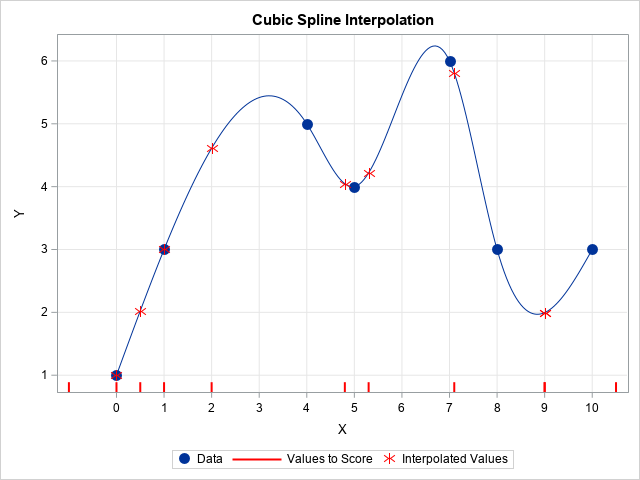
\includegraphics[width=0.95\linewidth]{cubicInterp1}\\[1mm]
\src{Cubic spline through sparse nodes.}
\end{column}
\begin{column}{0.50\textwidth}
\small
A cubic on each interval, matched in value, slope and curvature at every node: $C^{2}$ overall, error $O(h^{4})$.
\medskip

\textbf{Count the conditions.} $4(N-1)$ coefficients; $2(N-1)$ interpolation conditions, $N-2$ slope matches, $N-2$ curvature matches $=4N-6$. Two short --- hence the \emph{natural} ($\hat v''=0$ at the ends) or \emph{clamped} boundary conditions.
\medskip
\begin{cautionbox}\footnotesize
The same smoothness that buys $O(h^{4})$ is what makes it overshoot near a kink: the spline cannot turn sharply, so it swings past instead.
\end{cautionbox}
\end{column}
\end{columns}
\vspace{1mm}
\src{Adapted from QM Lec.~4, ``Cubic Spline'' frames (figure copied in) and QM Lec.~7 F24.}
\end{frame}

%=============================================================================
\begin{frame}{Shape-Preserving Schemes, and the Corrected Table}
\renewcommand{\arraystretch}{1.2}
\begin{center}\footnotesize
\begin{tabularx}{\linewidth}{@{}>{\raggedright\arraybackslash}p{2.6cm} c c c >{\raggedright\arraybackslash}X@{}}
\toprule
 & \textbf{accuracy} & \textbf{smooth} & \textbf{monotone} & \textbf{concavity} \\
\midrule
Linear & $O(h^{2})$ & $C^{0}$ & yes & \textbf{yes} \\
Cubic spline & $O(h^{4})$ & $C^{2}$ & no & no \\
PCHIP (Fritsch--Carlson) & $O(h^{3})$ & $C^{1}$ & \textbf{yes} & no \\
Schumaker & $O(h^{2})$ & $C^{1}$ & \textbf{yes} & \textbf{yes} \\
\bottomrule
\end{tabularx}
\end{center}
\vspace{1mm}
\begin{columns}[T]
\begin{column}{0.49\textwidth}
\begin{takeawaybox}\small
\textbf{Schumaker's quadratic spline} is the only row that preserves both, which is why it is the standard choice when a value function must stay concave.
\end{takeawaybox}
\end{column}
\begin{column}{0.48\textwidth}
\begin{cautionbox}\footnotesize
The published version of this table marks Linear as ``concavity: no''. Our measurement says otherwise, and the corrected entry is in bold. \textbf{Recompute the tables in your sources.}
\end{cautionbox}
\end{column}
\end{columns}
\vspace{1mm}
\src{Structure from QM Lec.~7, ``Interpolation: Comparison'' and ``Shape-Preserving Interpolation'', with the linear/concavity entry corrected.}
\end{frame}

%=============================================================================
\begin{frame}{More Than One Dimension}
\begin{columns}[c]
\begin{column}{0.44\textwidth}
\centering
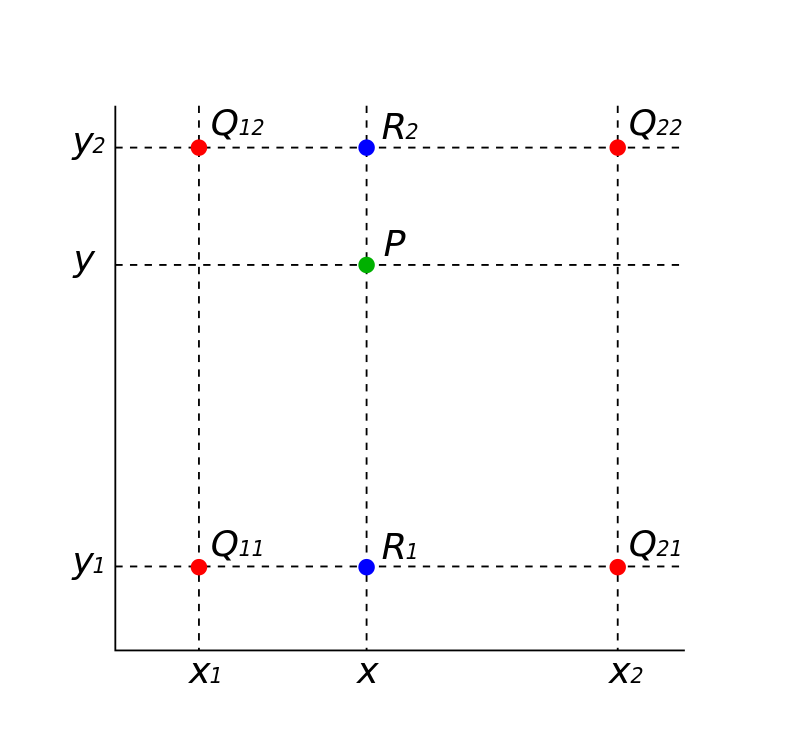
\includegraphics[width=0.88\linewidth]{bilinear_interpolation}\\[1mm]
\src{Bilinear interpolation on a rectangular cell.}
\end{column}
\begin{column}{0.53\textwidth}
\small
\textbf{Bilinear}: interpolate along $x$ on both edges, then along $y$ between the two results. Exact for $1,x,y,xy$; the natural extension of linear to a rectangular grid, and it keeps monotonicity in each argument separately.
\medskip

\textbf{Triangular (barycentric)}: split each cell into triangles and use weights $w_1,w_2,w_3\ge0$ summing to one. The interpolant is a genuine convex combination of the three vertices, so it \textbf{cannot overshoot} --- and it works on unstructured grids.
\medskip
\begin{cautionbox}\footnotesize
The cost is the real problem: a tensor grid needs $N^{d}$ points, which is 3.A3's curse arriving in the interpolation step rather than the maximization.
\end{cautionbox}
\end{column}
\end{columns}
\vspace{1mm}
\src{Adapted from QM Lec.~4, ``Bilinear'' and ``Triangular Interpolation'' frames; the bilinear figure is copied in and renamed (the source filename contains a dot and breaks SVG-aware drivers).}
\end{frame}

%=============================================================================
\begin{frame}{Smolyak: Most of a Tensor Grid Is Wasted}
\begin{columns}[T]
\begin{column}{0.52\textwidth}
\small
A tensor grid takes every combination of one-dimensional nodes, so it spends points on corners where \emph{every} coordinate is extreme at once --- states the model almost never visits.
\medskip

\textbf{Smolyak's construction} keeps only the combinations whose total resolution is modest. With one-dimensional node sets $G^{1},G^{2},\dots$ indexed by $i_1,\dots,i_d$, take the union of tensor products over a \emph{budget} on the index sum,
\[
  \Phi(q,d)=\!\!\bigcup_{q-d+1\le|i|\le q}\!\!\big(G^{i_1}\!\times\cdots\times G^{i_d}\big),
\]
writing $|i|=\sum_j i_j$ and $q=d+\mu$. High resolution in \emph{one} dimension is allowed; high resolution in all of them at once is not. $\mu$ is the \textbf{level}: $\mu=0$ is a single point.
\end{column}
\begin{column}{0.45\textwidth}
\begin{center}\footnotesize
\begin{tabularx}{\linewidth}{@{}c r r r@{}}
\toprule
$d$ & \textbf{Smolyak $\mu{=}2$} & \textbf{$5^{d}$} & \textbf{$9^{d}$} \\
\midrule
2 & 13 & 25 & 81 \\
3 & 25 & 125 & 729 \\
4 & 41 & 625 & 6{,}561 \\
5 & 61 & 3{,}125 & 59{,}049 \\
10 & \textbf{221} & \textbf{9.8 million} & $3.5\times10^{9}$ \\
12 & 313 & 244 million & $2.8\times10^{11}$ \\
\bottomrule
\end{tabularx}
\end{center}
\vspace{1mm}
\begin{takeawaybox}\footnotesize
At ten dimensions the sparse grid needs \textbf{221 points} where a five-point tensor grid needs nearly ten million --- a factor of \textbf{44{,}000}.
\end{takeawaybox}
\end{column}
\end{columns}
\vspace{1mm}
\src{Smolyak (1963); in economics Krueger \& Kubler (2004), Malin, Krueger \& Kubler (2011), Judd, Maliar, Maliar \& Valero (2014). Our run reproduces Malin--Krueger--Kubler's own table at $\mu=2$ exactly: $d=2,4,5,12 \Rightarrow 13, 41, 61, 313$.}
\end{frame}

%=============================================================================
\begin{frame}{The Ladder: Nested Node Sets, and Why Nesting Is the Point}
\begin{columns}[T]
\begin{column}{0.53\textwidth}
\small
The one-dimensional sets are not arbitrary. Take
\[
  m_1=1,\qquad m_i=2^{\,i-1}+1 ,
\]
and let $G^{i}$ be the $m_i$ \textbf{extrema} of a Chebyshev polynomial,
\[
  x^{i}_{j}=-\cos\!\Big(\frac{\pi(j-1)}{m_i-1}\Big),\quad j=1,\dots,m_i ,
\]
with $G^{1}=\{0\}$ by convention.
\medskip
\begin{center}\footnotesize
\begin{tabularx}{\linewidth}{@{}c c >{\raggedright\arraybackslash}X@{}}
\toprule
$i$ & $m_i$ & $G^{i}$ \\
\midrule
1 & 1 & $\{0\}$ \\
2 & 3 & $\{-1,\,0,\,1\}$ \\
3 & 5 & $\{-1,\,-0.7071,\,0,\,0.7071,\,1\}$ \\
4 & 9 & $\{\pm1,\pm0.9239,\pm0.7071,\pm0.3827,0\}$ \\
\bottomrule
\end{tabularx}
\end{center}
\end{column}
\begin{column}{0.44\textwidth}
\begin{conceptbox}[title=\textbf{$G^{1}\subset G^{2}\subset G^{3}\subset\cdots$}]\small
\textbf{Checked in the run: every level contains the one below it.} That is the property the whole construction rests on.
\end{conceptbox}
\vspace{-1mm}
\begin{takeawaybox}\footnotesize
Nesting buys two things. The union that defines $\Phi$ is mostly \textbf{overlap}, so the point count grows far more slowly than the number of index sets; and \textbf{refining the grid reuses every function value you already paid for} --- going from $\mu$ to $\mu+1$ adds points, it does not move them.
\end{takeawaybox}
\vspace{-1mm}
\begin{cautionbox}\footnotesize
Equally spaced nodes are \emph{not} nested this way, and Chebyshev \emph{zeros} are not either. The extrema are chosen for exactly this reason.
\end{cautionbox}
\end{column}
\end{columns}
\end{frame}

%=============================================================================
\begin{frame}{Building It in Two Dimensions, By Hand}
\begin{columns}[c]
\begin{column}{0.51\textwidth}
\centering
\begin{tikzpicture}
\begin{axis}[
    width=6.6cm, height=6.0cm, xmin=-1.22, xmax=1.22, ymin=-1.22, ymax=1.22,
    xtick={-1,0,1}, ytick={-1,0,1},
    tick label style={font=\scriptsize},
    axis x line*=bottom, axis y line*=left,
    legend style={font=\tiny, draw=none, fill=none,
                  at={(0.5,-0.22)}, anchor=north, legend columns=2}]
  \addplot[only marks, mark=o, mark size=1.9pt, black!45] coordinates {(-1.0000,-1.0000) (-1.0000,-0.7071) (-1.0000,-0.0000) (-1.0000,0.7071) (-1.0000,1.0000) (-0.7071,-1.0000) (-0.7071,-0.7071) (-0.7071,-0.0000) (-0.7071,0.7071) (-0.7071,1.0000) (-0.0000,-1.0000) (-0.0000,-0.7071) (-0.0000,-0.0000) (-0.0000,0.7071) (-0.0000,1.0000) (0.7071,-1.0000) (0.7071,-0.7071) (0.7071,-0.0000) (0.7071,0.7071) (0.7071,1.0000) (1.0000,-1.0000) (1.0000,-0.7071) (1.0000,-0.0000) (1.0000,0.7071) (1.0000,1.0000)};
  \addlegendentry{tensor $5\times5$ (25)}
  \addplot[only marks, mark=*, mark size=2.1pt, RedTitle] coordinates {(-1.0000,-1.0000) (-1.0000,0.0000) (-1.0000,1.0000) (-0.7071,0.0000) (0.0000,-1.0000) (0.0000,-0.7071) (0.0000,0.0000) (0.0000,0.7071) (0.0000,1.0000) (0.7071,0.0000) (1.0000,-1.0000) (1.0000,0.0000) (1.0000,1.0000)};
  \addlegendentry{Smolyak $\mu=2$ (13)}
\end{axis}
\end{tikzpicture}
\end{column}
\begin{column}{0.46\textwidth}
\small
\textbf{$\mu=0$:} only $i_1+i_2\le2$, so $(1,1)$ alone and $\Phi=\{(0,0)\}$ --- one point.
\medskip

\textbf{$\mu=1$:} $2\le i_1+i_2\le3$ admits $(1,1),(1,2),(2,1)$, and the union is the five-point cross
\[
  \{(0,0),(\pm1,0),(0,\pm1)\} .
\]
\textbf{$\mu=2$:} adds $(1,3),(2,2),(3,1)$ --- \textbf{13} of the 25 tensor points.
\medskip
\begin{cautionbox}\footnotesize
Notice \emph{which} 12 are dropped: every point with two non-central coordinates except the four corners. The sparse grid keeps the \textbf{axes and the corners} and throws away the interior cross-terms.
\end{cautionbox}
\end{column}
\end{columns}
\end{frame}

%=============================================================================
\begin{frame}{Three Dimensions, and the Signed Combination}
\begin{columns}[T]
\begin{column}{0.47\textwidth}
\small
At $d=3$, $\mu=2$ the admissible multi-indices are the ten
\[
\begin{array}{lll}
(1,1,1) & (1,1,2) & (1,2,1)\\
(2,1,1) & (1,1,3) & (1,2,2)\\
(1,3,1) & (2,1,2) & (2,2,1)\\
(3,1,1) & &
\end{array}
\]
whose union is \textbf{25 distinct points}, against $5^{3}=125$.
\medskip

The approximation is \emph{not} a plain interpolation on those points. It is a signed combination of tensor interpolants,
\[
  \hat f=\!\!\sum_{q-d+1\le|i|\le q}\!\!(-1)^{q-|i|}\binom{d-1}{q-|i|}\,
  \big(U^{i_1}\!\otimes\cdots\otimes U^{i_d}\big),
\]
which cancels the overlaps the union created.
\end{column}
\begin{column}{0.50\textwidth}
\begin{center}\footnotesize
\textbf{Coefficients at $d=2$, $\mu=2$ ($q=4$)}\\[1mm]
\begin{tabularx}{\linewidth}{@{}c c r@{}}
\toprule
$i$ & $|i|$ & $(-1)^{q-|i|}\binom{d-1}{q-|i|}$ \\
\midrule
$(1,1)$ & 2 & \textbf{0} \\
$(1,2)$, $(2,1)$ & 3 & $-1$ \\
$(1,3)$, $(2,2)$, $(3,1)$ & 4 & $+1$ \\
\bottomrule
\end{tabularx}
\end{center}
\vspace{1mm}
\begin{examplebox}\footnotesize
The zero explains why the two index ranges you see in the literature --- $d\le|i|\le q$ and $q-d+1\le|i|\le q$ --- give the same answer: the extra terms have coefficient $\binom{d-1}{q-|i|}=0$, and by nesting they add no points either.
\end{examplebox}
\vspace{-2mm}
\begin{cautionbox}\footnotesize
\textbf{Signed} weights: a sparse \emph{quadrature} rule built this way can have negative ones, so it need not be positive --- unlike Gauss rules (4.B2).
\end{cautionbox}
\end{column}
\end{columns}
\vspace{-1mm}
\src{Construction and the $d=3$ list from Malin, Krueger \& Kubler (2011). Their example frame labels it $\Phi(5,2)$; with $d=3,\mu=2$ it is $\Phi(5,3)$.}
\end{frame}

%=============================================================================
\begin{frame}{What Sparsity Costs, and Where It Reappears}
\begin{columns}[T]
\begin{column}{0.52\textwidth}
\small
Nothing is free. The sparse grid is exact for a \textbf{smaller} set of polynomials than the tensor grid it replaces --- roughly the \emph{total-degree} set rather than the full tensor set --- so it loses the cross-terms of highest order. For $f\in C^{k}$ the error is bounded by
\[
  C_{d}\,n^{-k}\,(\log n)^{(d-1)(k+1)}\lVert f\rVert_{k},
\]
$n=|\Phi(q,d)|$: the tensor rate $n^{-k}$, spoiled by a $\log$ factor that grows with $d$. \textbf{The curse is weakened, not broken.}
\medskip

That is usually the right trade in economics, because the functions we approximate are smooth and their high-order interactions are small. It is the wrong trade when the object has a \textbf{kink} whose position depends on several states at once --- a borrowing constraint that binds only for the young and unlucky.
\end{column}
\begin{column}{0.45\textwidth}
\begin{conceptbox}[title=\textbf{Two uses, one construction}]\small
Here Smolyak is a \textbf{node set} --- where to evaluate a function you are interpolating, and where to place quadrature nodes.\\[1mm]
In \textbf{Session 5} it becomes a \textbf{basis}: the same index rule selects which polynomials enter a projection method, and the coefficients are chosen to kill a residual.
\end{conceptbox}
\medskip
\begin{examplebox}\footnotesize
Same combinatorics, different job. Worth keeping the distinction straight, because the literature uses ``Smolyak'' for both.
\end{examplebox}
\end{column}
\end{columns}
\end{frame}

%=============================================================================
\begin{frame}{Global Polynomials, and Why Equally Spaced Nodes Fail}
\begin{columns}[c]
\begin{column}{0.52\textwidth}
\centering
\begin{tikzpicture}
\begin{axis}[
    width=7.6cm, height=5.3cm, xmin=3, xmax=23, ymin=-2.2, ymax=2.2,
    xlabel={\scriptsize number of nodes $n$}, ylabel={\scriptsize $\log_{10}$ max error},
    tick label style={font=\scriptsize}, xtick={5,9,15,21},
    axis x line*=bottom, axis y line*=left,
    legend style={font=\tiny, draw=none, fill=none, at={(0.02,0.03)}, anchor=south west}]
  \addplot[very thick, RedTitle, mark=*, mark size=1.3pt] coordinates {(5,-0.358) (9,0.019) (15,0.857) (21,1.777)};
  \addlegendentry{equally spaced}
  \addplot[very thick, orange!80!black, mark=square*, mark size=1.2pt] coordinates {(5,-0.396) (9,-0.767) (15,-1.332) (21,-1.814)};
  \addlegendentry{Chebyshev nodes}
  \draw[black!45, dashed] (axis cs:3,0) -- (axis cs:23,0);
\end{axis}
\end{tikzpicture}
\end{column}
\begin{column}{0.45\textwidth}
\small
Interpolate Runge's function $1/(1+25x^{2})$ on $[-1,1]$ by a single polynomial through $n$ nodes.
\medskip
\begin{center}\footnotesize
\begin{tabularx}{\linewidth}{@{}c r r@{}}
\toprule
$n$ & \textbf{equispaced} & \textbf{Chebyshev} \\
\midrule
5 & 0.44 & 0.40 \\
9 & 1.05 & 0.17 \\
15 & 7.19 & 0.047 \\
21 & \textbf{59.8} & \textbf{0.015} \\
\bottomrule
\end{tabularx}
\end{center}
\medskip
\begin{cautionbox}\footnotesize
More points makes the equispaced fit \textbf{worse}, by a factor of 136 between $n=5$ and $n=21$. The oscillation is at the ends, and it diverges.
\end{cautionbox}
\end{column}
\end{columns}
\end{frame}

%=============================================================================
\begin{frame}{Chebyshev Nodes: Cluster at the Ends}
\begin{columns}[T]
\begin{column}{0.53\textwidth}
\small
On $[-1,1]$,
\[
  x_i=\cos\!\Big(\frac{2i-1}{2n}\pi\Big), \qquad i=1,\dots,n,
\]
mapped to $[a,b]$ by $s_i=\tfrac{a+b}{2}+\tfrac{b-a}{2}x_i$. These nodes \textbf{minimise the maximum} interpolation error over all node choices, and they are dense exactly where the equispaced fit blew up --- at the boundaries.
\medskip

At $n=21$ the Chebyshev error is $0.015$ against the equispaced $59.8$: \textbf{four thousand times better}, with the same number of points and the same degree.
\end{column}
\begin{column}{0.44\textwidth}
\begin{cautionbox}[title=\textbf{Read the formula carefully}]\small
$i=1$ gives $\cos(\pi/2n)$, which is close to $+1$. The nodes come out \textbf{descending}.\\[1mm]
Every routine downstream --- a monotonicity ratchet, a bracketing search, \texttt{np.interp} --- assumes an ascending grid. \textbf{Sort them.}
\end{cautionbox}
\medskip
\begin{examplebox}\footnotesize
This is the one line of this deck that students reliably get wrong the first time they code it, and the failure is silent.
\end{examplebox}
\end{column}
\end{columns}
\vspace{1mm}
\src{Node formula and minimax property from QM Lec.~7, ``Chebyshev Nodes''; the ordering warning is ours.}
\end{frame}

%=============================================================================
\begin{frame}{Where Polynomials Cannot Be Rescued: Gibbs}
\begin{columns}[T]
\begin{column}{0.52\textwidth}
\small
Runge's problem is fixed by moving the nodes. A genuine \textbf{discontinuity} is not.
\medskip

Fit a degree-20 polynomial to a step function and it overshoots by $0.41$ --- on a jump of size one. Raise the degree and the overshoot \emph{does not shrink}; it merely moves closer to the jump. That is the Gibbs phenomenon, and it is a property of the approximating family, not of the fit.
\end{column}
\begin{column}{0.45\textwidth}
\begin{takeawaybox}[title=\textbf{What to do instead}]\small
Use a \textbf{local} scheme, or split the domain at the kink and approximate each piece separately.\\[1mm]
Economics produces kinks routinely: borrowing constraints, occasionally binding bounds, discrete choices.
\end{takeawaybox}
\medskip
\begin{cautionbox}\footnotesize
A neural network is also a global approximator --- but with a \emph{kinked} basis, which is why ReLU networks handle these problems more gracefully (S7).
\end{cautionbox}
\end{column}
\end{columns}
\vspace{1mm}
\src{Gibbs discussion adapted from QM Lec.~5, ``Case Study: Fitting Data''; overshoot measured here.}
\end{frame}

%=============================================================================
\begin{frame}{Takeaways}
\begin{takeawaybox}
\begin{itemize}\small
  \item Interpolation is not a detail of a dynamic program --- it is inside the fixed point, so its error \textbf{compounds through every sweep}.
  \item \textbf{Linear interpolation preserves concavity}, contrary to the table everyone prints, and that is precisely what licenses golden section inside the Bellman loop.
  \item Cubic splines buy $O(h^{4})$ and lose shape. On a capped policy the spline \textbf{overshot the cap by 0.043} and broke both monotonicity and concavity; linear interpolation was exact.
  \item Equally spaced nodes make a global polynomial \textbf{worse} as you add points --- error 0.44 to 59.8 from $n=5$ to $21$. Chebyshev nodes fix it; at $n=21$ they are four thousand times better.
  \item $x_i=\cos((2i-1)\pi/2n)$ comes out \textbf{descending}. Sort it.
  \item A discontinuity cannot be fixed by moving nodes. \textbf{Gibbs does not go away} --- go local, or split the domain.
  \item In several dimensions a tensor grid is mostly waste. \textbf{Smolyak} needs 221 points in ten dimensions where a five-point tensor grid needs 9.8 million --- and it returns in Session 5 as a \emph{basis} rather than a node set.
\end{itemize}
\end{takeawaybox}
\end{frame}

%=============================================================================
\begin{frame}{Bridge: The Other Thing a Grid Cannot Do}
\begin{columns}[T]
\begin{column}{0.53\textwidth}
\small
We can now represent $\hat v$ between grid points and know which schemes keep the properties the algorithms need.
\medskip

But the Bellman equation does not only evaluate $\hat v$ --- it takes an \textbf{expectation} of it:
\[
  \mathbb{E}\big[\hat v(k',z')\,\big|\,z\big]=\int \hat v(k',z')\,dF(z'\mid z).
\]
Every solve so far has replaced that integral with a finite sum $\sum_m \Pi_{jm}\hat v(k',z_m)$ --- and we have written $\Pi$ down by hand twice now, without ever saying where it comes from.
\end{column}
\begin{column}{0.44\textwidth}
\begin{conceptbox}[title=\textbf{Next (4.B2)}]\small
Quadrature: how an integral becomes a finite sum, and how much accuracy the choice of rule is worth.\\[1mm]
Then \textbf{4.B3} answers the question directly --- where $\Pi$ comes from, and which of the two standard constructions you should actually use.
\end{conceptbox}
\end{column}
\end{columns}
\end{frame}

\end{document}
